\section{Data organisation} \label{gt}
This section demonstrates how we organised the actual storage of all the different data we collected in order to exploit them in the most efficient way.

\subsection{Storage}
Our first thought was to store our data directly in CSV files. This format is easy to use, requires no installation or additional software and is very lightweight. However, if we want to retrieve any other kinds of information, such as the number of malware analysed in March or how many samples are considered as packed by Cisco, we will quickly find ourselves limited. That's why we came up with the idea of using a database, knowing that it presents the following advantages:

\begin{itemize}
    \item \textbf{Modularity:} we take advantage of the links between the tables to easily add a detector or any entry in the tables.
    \item \textbf{Retrieval:} we can use the \texttt{SQL} language to create powerful queries among our data, for example to find duplicates, malware that have not yet been scanned and so on.
    \item \textbf{Accessibility} : the database is available through the internet and allows the management of several users. The software we designed in the previous section is continuously adding new entries so that we can keep doing queries in the meantime.
\end{itemize}

\subsection{Exportation}

With so many data stored in the database, the next step is to take advantage of such an organisation and generate interesting datasets to carry out our further experiments. We wrote a script that takes several parameters to vary the output, the goal being to generate a CSV file containing the dataset with the desired options. As we cannot determine when new data are added to our system because of its full automation, the generation of an intermediate CSV allows to produce snapshots of the database. They keep a combination of the different parameters that were requested and the date when the request was made. By using the same CSV file for each machine learning algorithm, we are sure that they will work on the same data and that no other inputs were added between two executions. Doing this allows to compare the classifiers among the same dataset. 

As one could have understood, from now on we make the strong assumption that the datasets we generate are valid, i.e. that samples labeled as packed are actually packed. This is a fundamental hypothesis as all further machine learnings are based on these datasets, also called ground truths.

The main purpose of the script generating the different ground truths is also to merge the results of our 5 detectors into one final decision. This is achieved by using the notion of threshold which can have a value between 1 and 5. As soon as the number of detectors that consider a malware as packed reaches the threshold, then the sample is labeled as packed. As shown in table \ref{fig:agreements}, the number of results that are positive is greater than or equal to the imposed threshold of 3, the malware is then officially considered as packed. 

\begin{table}[h]
    \centering
    \begin{tabular}{|c|c|c|c|c|c|}
    \hline
     Peframe & Manalyze & PEiD & DIE & Cisco & Decision \\
    \hline
     UPX & none & UPX & PEtite & none & \textbf{packed} \\
    \hline
    \end{tabular}
    \caption{Decision with a threshold of 3/5}
    \label{fig:agreements}
\end{table}


% Below we list the following options that can be configured when asking the \textit{csv\_dump.py} script to generate a new dataset:

% \begin{itemize}
%  \item \textbf{--agreement} When this option is specified, the detectors must detect the same packer and not just consider the malware as packed. In figure \ref{fig:agreement}, the malware is no longer considered as packed since all 3 detectors do not agree on the same packer name.
% \item \textbf{-a, --array} This option is followed by an array containing the features you wish to have in the CSV among the 119 available.
% \item \textbf{--boolean} Returns only boolean features.
% \item \textbf{-e, --error} When a detector encounters a problem analysing a malware, it will indicate \texttt{error} in the database instead of the result. This option allows to consider errors as positive results.
% \item \textbf{-l, --limit} Specifies the size of the resulting CSV in terms of number of samples.
% \item \textbf{-t, --threshold} As explained above, a malware is considered as packed if it is considered as such by several detectors. This parameter makes it possible to change the threshold value. By default, the value is set to 3.
% \item \textbf{-s, --start} It is possible to choose the start date of the analysis. This can be useful to perform analysis through different periods of time. The expected format is \textbf{YYYYMMDD}. As an example, June 6, 2020 will be written as 20200606.

%  \end{itemize}

\subsection{Visualisation}
To facilitate the visualisation of the data and the progression of the analysis, we created a web interface. Thanks to this application, we can view all malware by date. By clicking on the hash of a malware, the result of the detectors as well as the feature values are displayed.

\begin{figure}[!hb]
\centering
  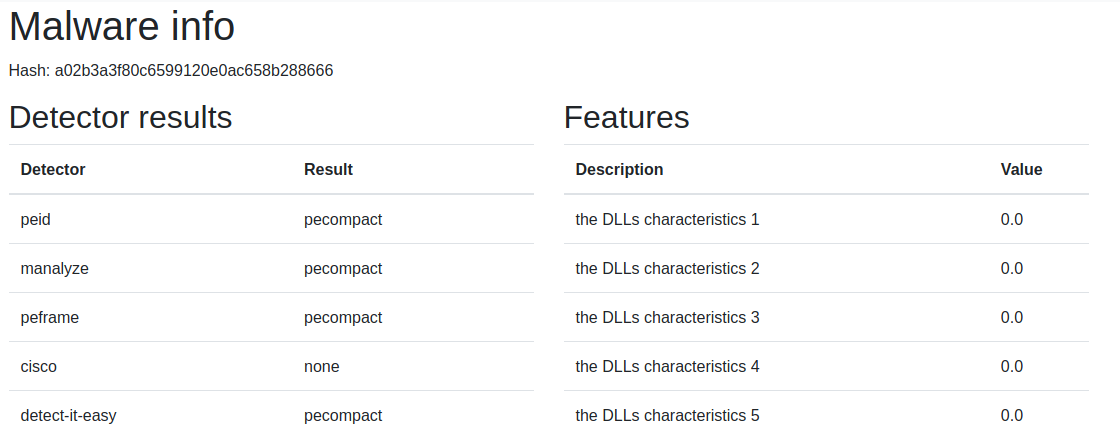
\includegraphics[width=0.9\linewidth]{Figures/malware_info.png}
  \caption{Malware information available via a web interface}
  \label{fig:KNN}
\end{figure}